\clearpage
\section{Trigger efficiency measurements of alphaT triggers \label{app:alphaTTriggerEfficiencies}}

Illustrative turn-ons of the individual \scalht-\alphat triggers as a function of \alt and \scalht, following the full signal region selection, using the \verb!HLT_Ele23_eta2p1_WPLoose_Gsf! reference trigger.

\begin{figure}[h!]
  \begin{center}
    \subfigure[{\tiny HLT\_PFHT200\_DiPFJetAve90\_PFAlphaT0p57 ($\scalht>300$~GeV)}]{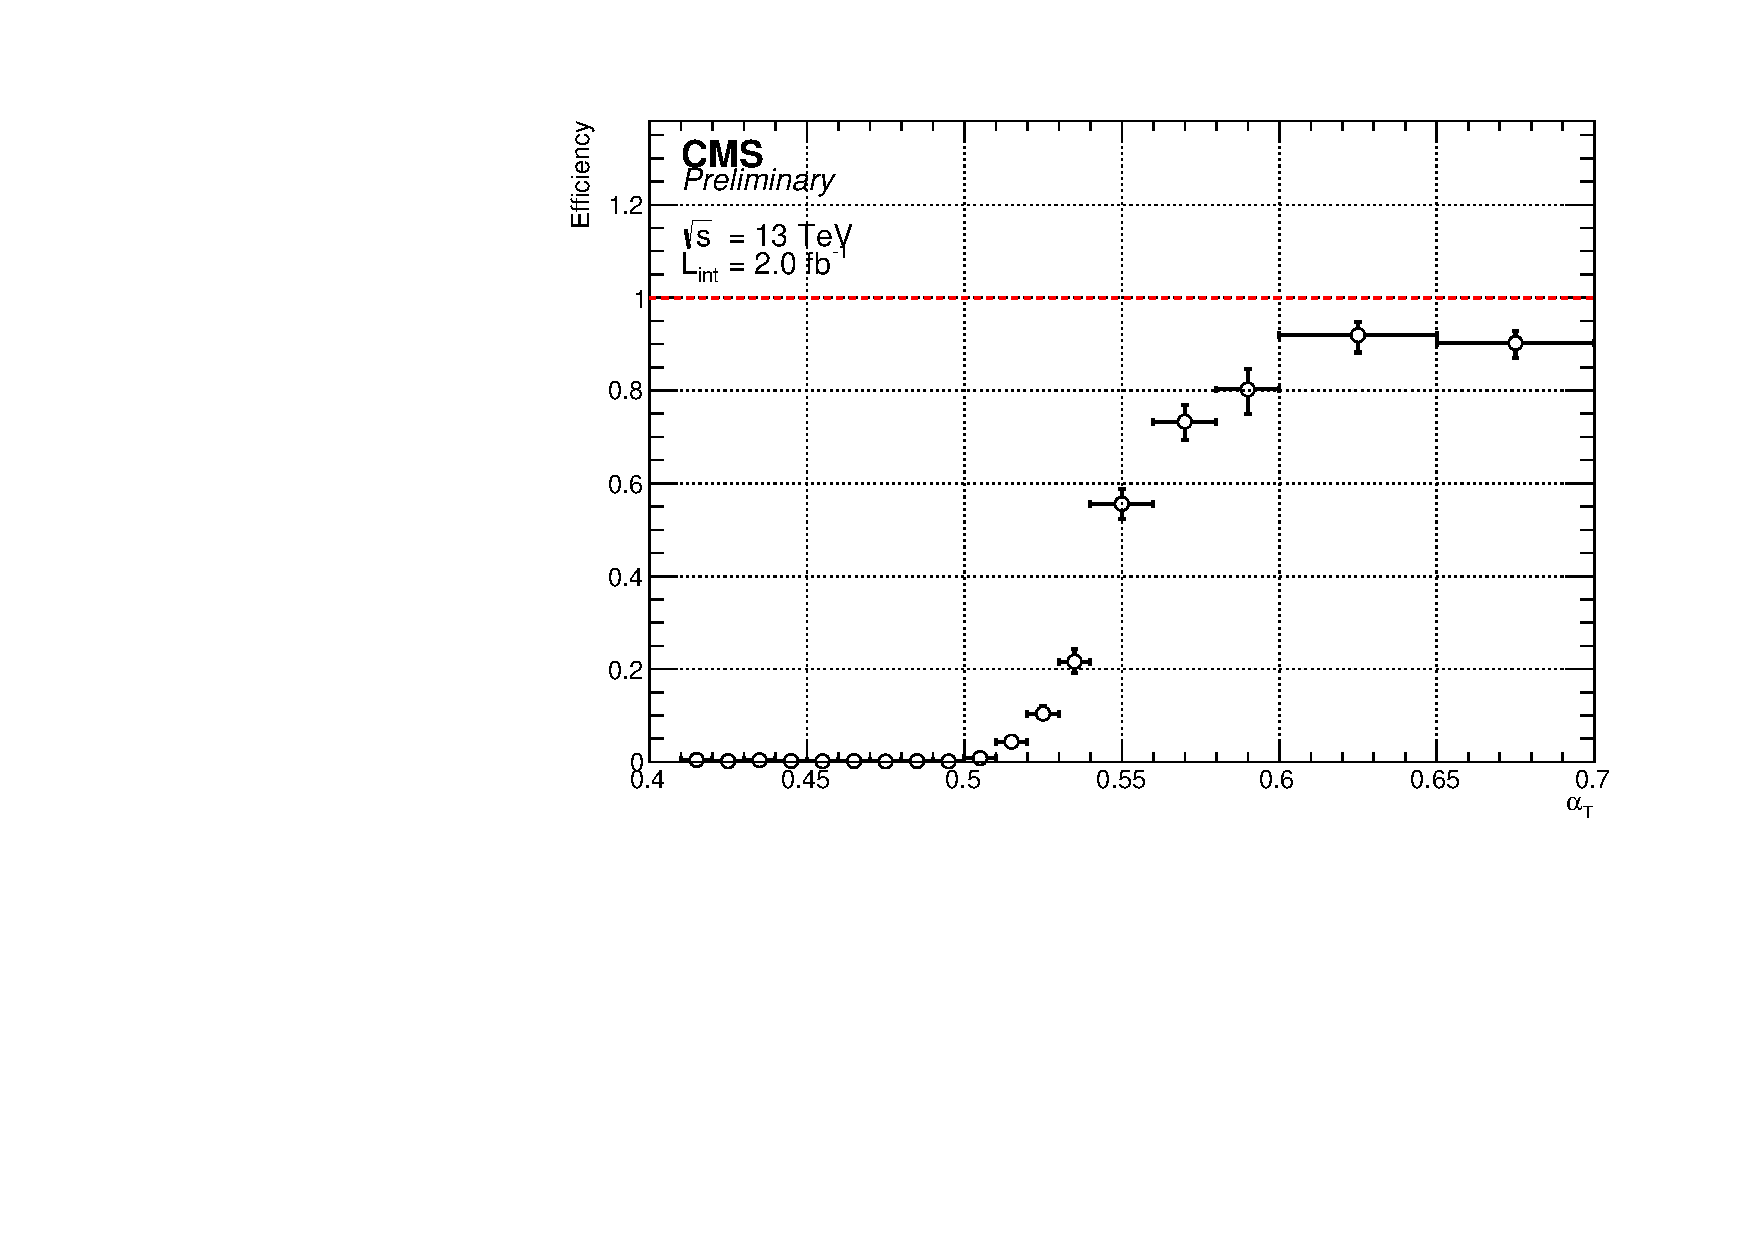
\includegraphics[width=0.5\textwidth]{figures/Trigger/HLT_Ele23_eta2p1_WPLoose_Gsf/HLT_PFHT200_DiPFJetAve90_PFAlphaT0p57_MoM_HT300_alphaT}} ~~
    \subfigure[{\tiny HLT\_PFHT200\_DiPFJetAve90\_PFAlphaT0p57 ($\alt>0.60$)}]{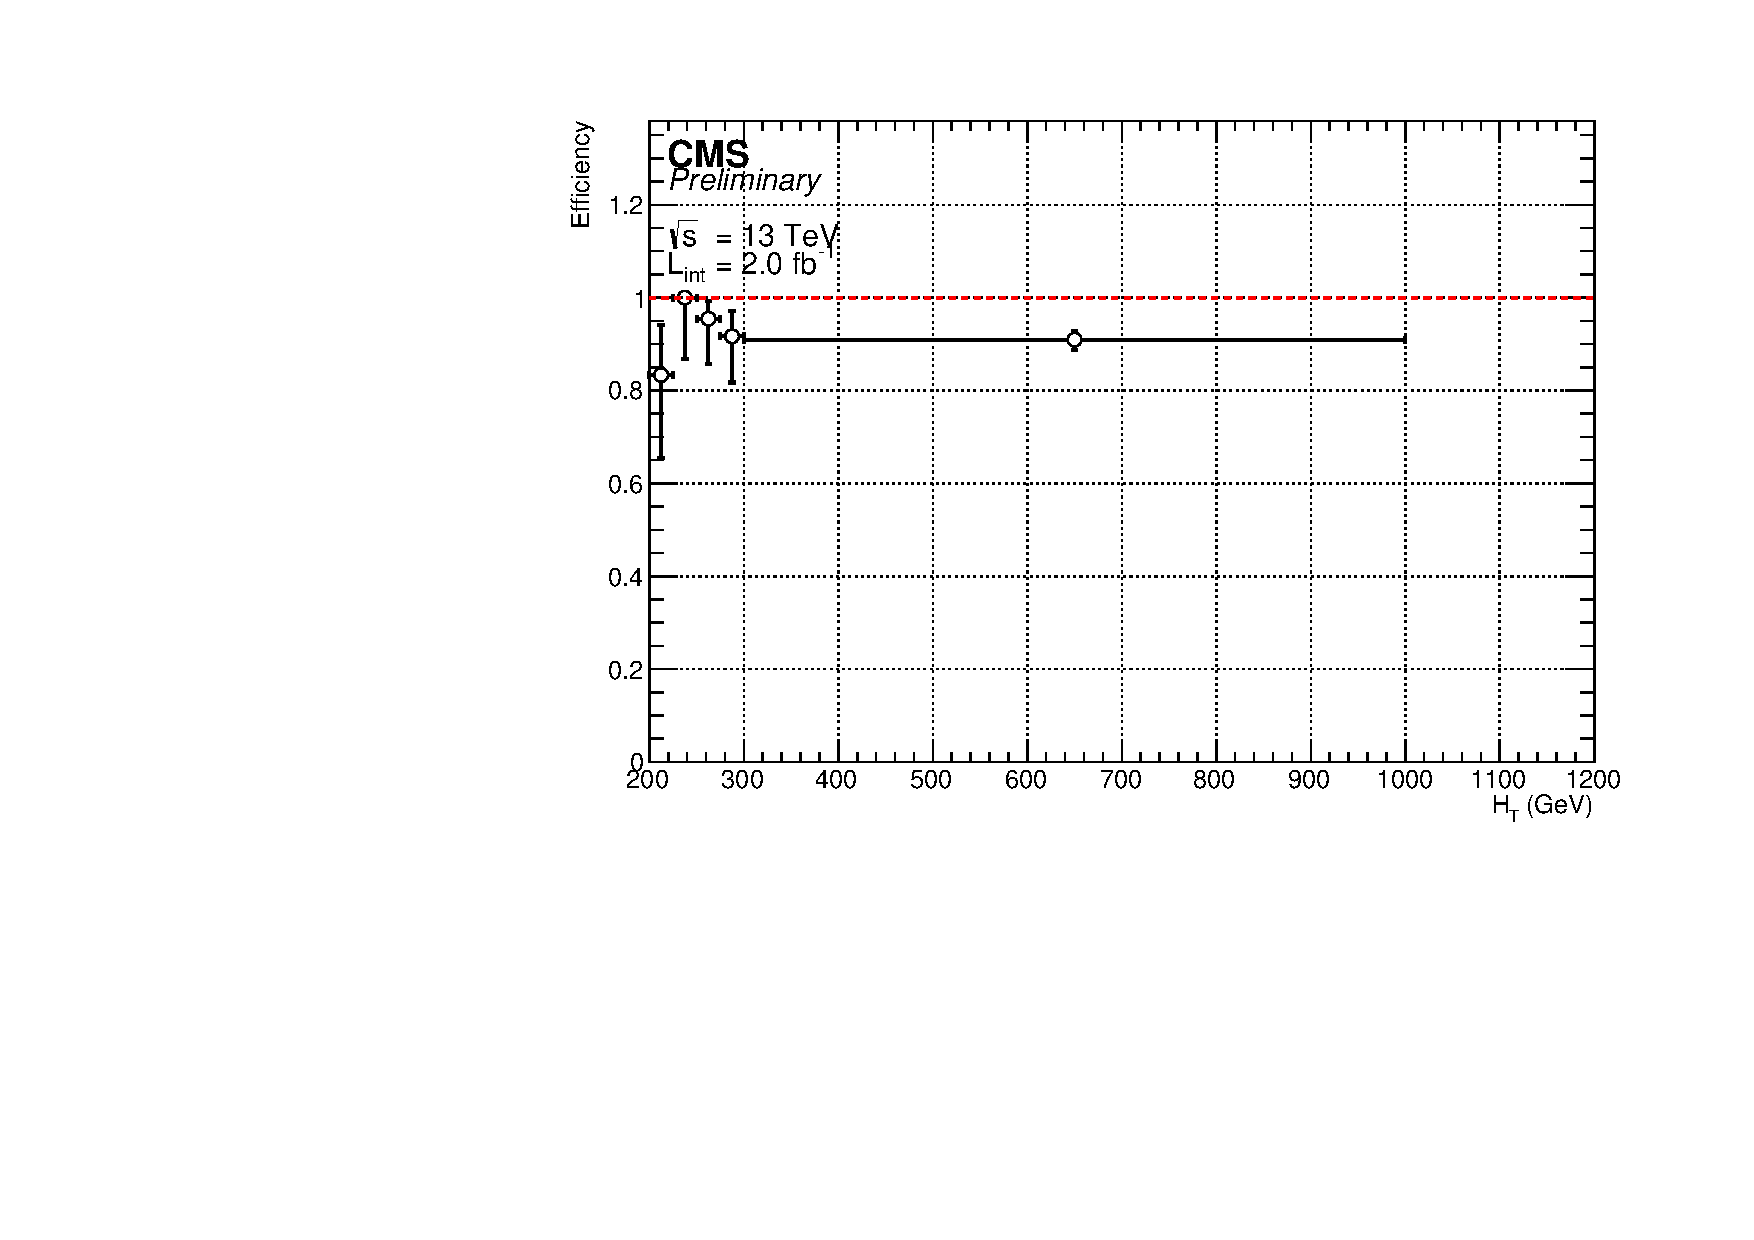
\includegraphics[width=0.5\textwidth]{figures/Trigger/HLT_Ele23_eta2p1_WPLoose_Gsf/HLT_PFHT200_DiPFJetAve90_PFAlphaT0p57_MoM_aT0p60_ht}} \\
    \subfigure[{\tiny HLT\_PFHT300\_DiPFJetAve90\_PFAlphaT0p53 ($\scalht>400$~GeV)}]{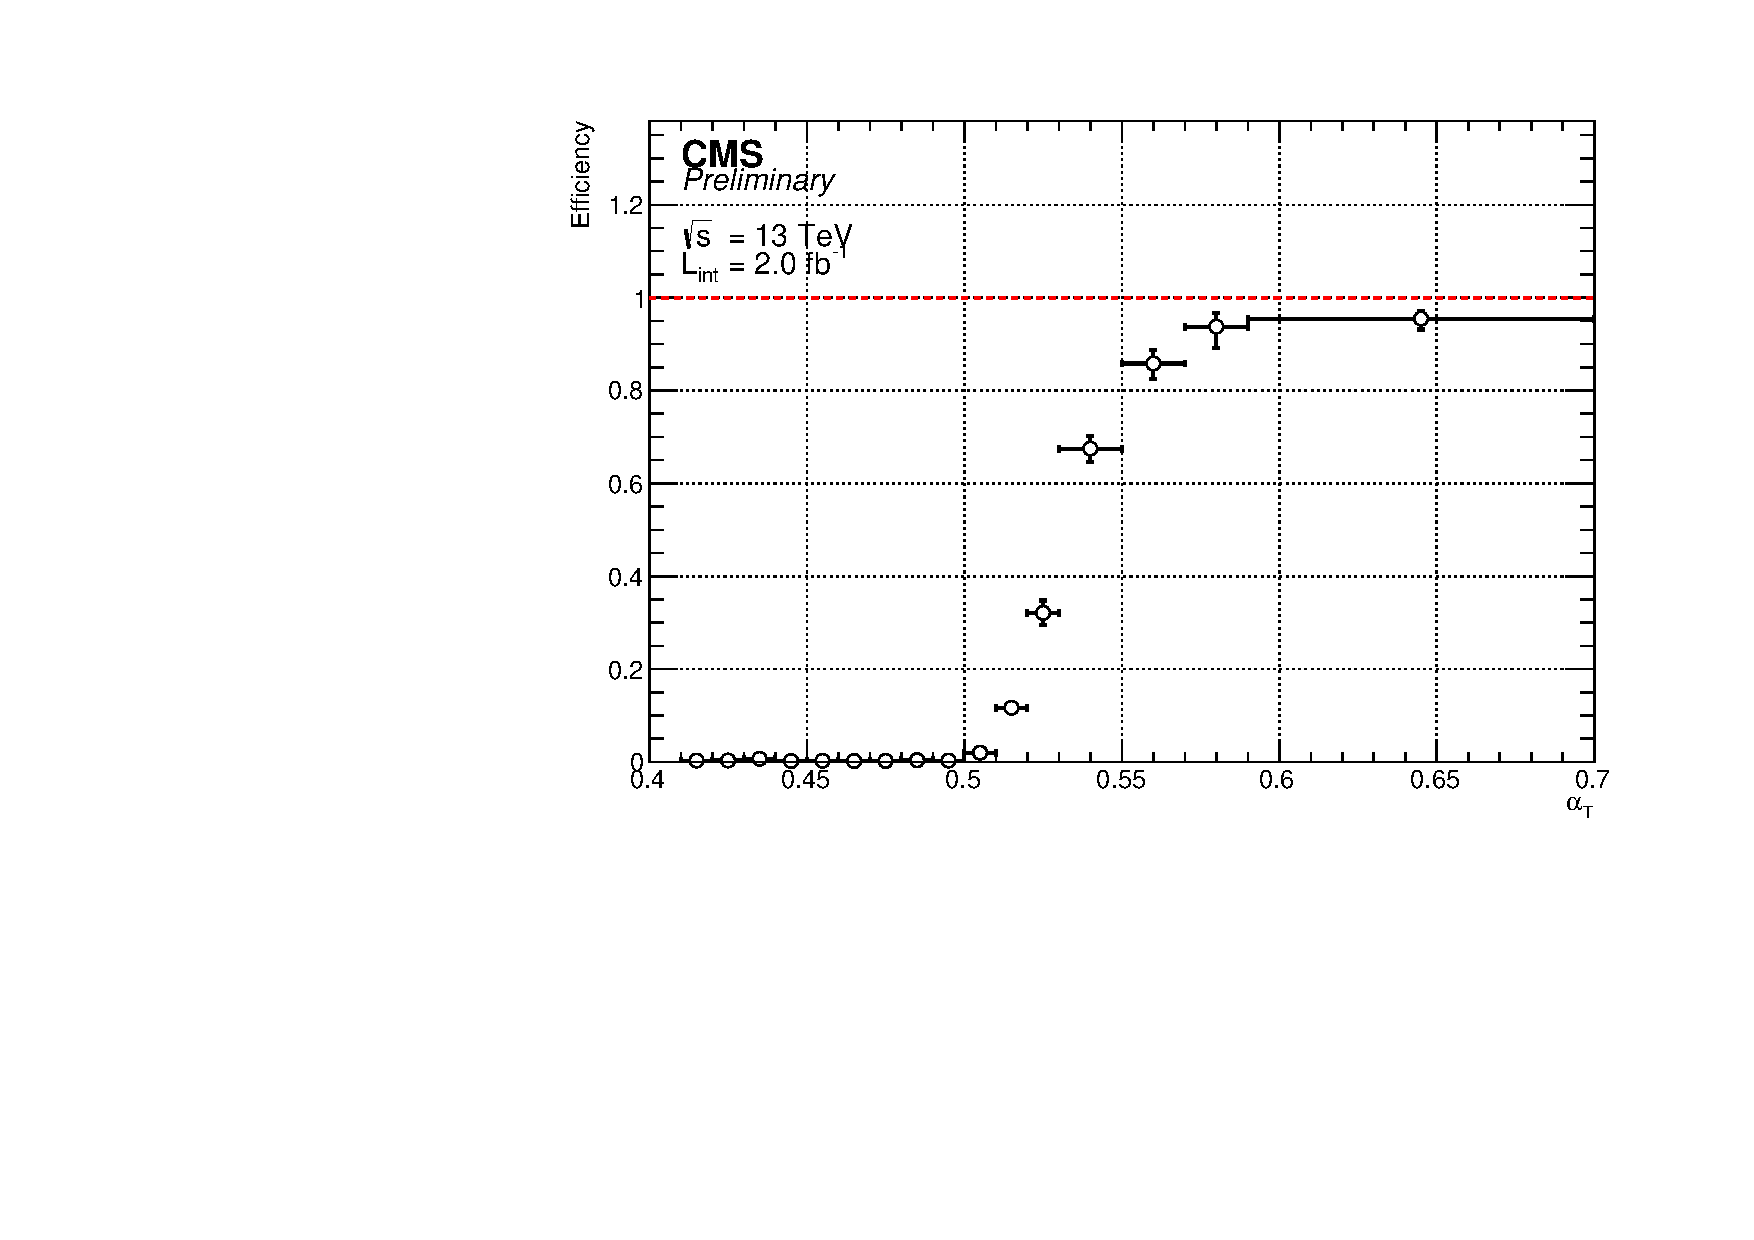
\includegraphics[width=0.5\textwidth]{figures/Trigger/HLT_Ele23_eta2p1_WPLoose_Gsf/HLT_PFHT300_DiPFJetAve90_PFAlphaT0p53_MoM_HT400_alphaT}} ~~
    \subfigure[{\tiny HLT\_PFHT300\_DiPFJetAve90\_PFAlphaT0p53 ($\alt>0.58$)}]{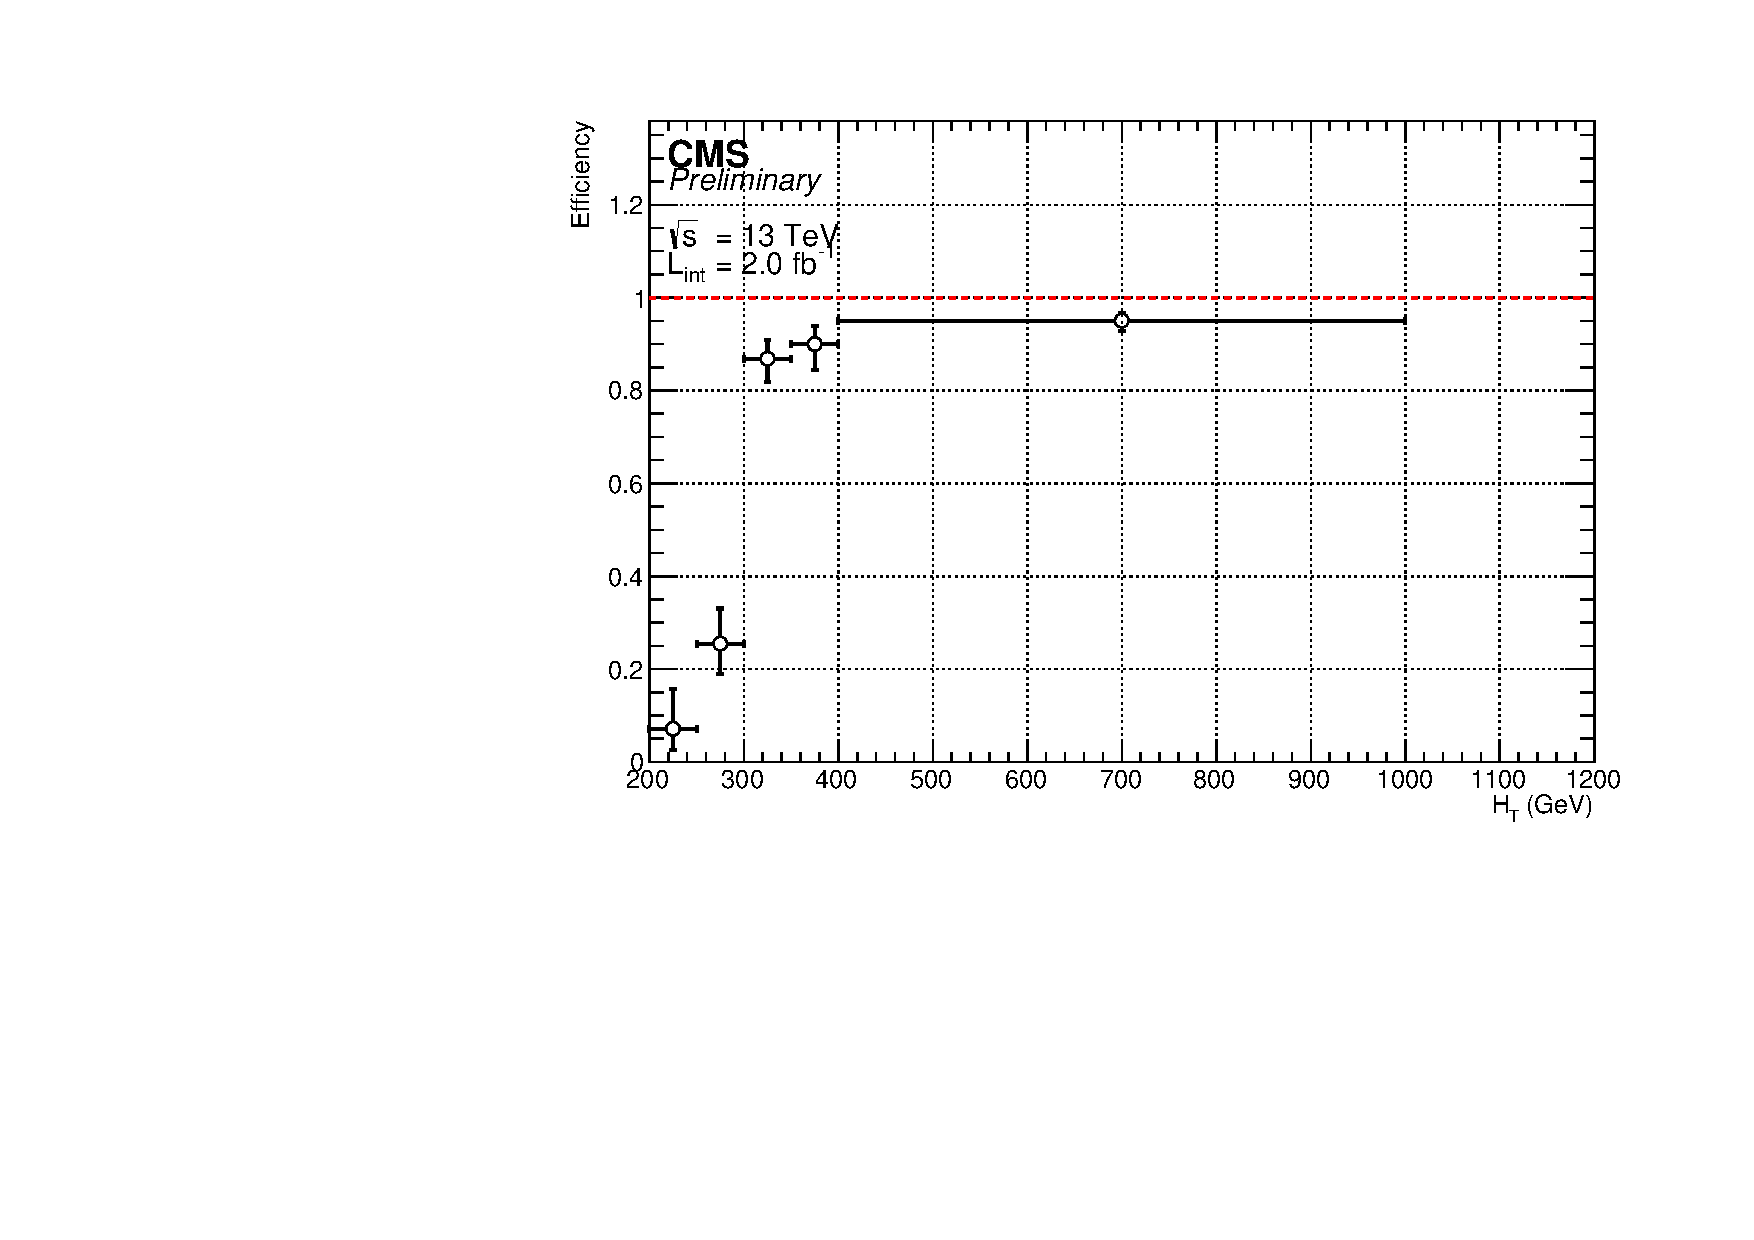
\includegraphics[width=0.5\textwidth]{figures/Trigger/HLT_Ele23_eta2p1_WPLoose_Gsf/HLT_PFHT300_DiPFJetAve90_PFAlphaT0p53_MoM_aT0p58_ht}} \\
    \subfigure[{\tiny HLT\_PFHT400\_DiPFJetAve90\_PFAlphaT0p51 ($\scalht>500$~GeV)}]{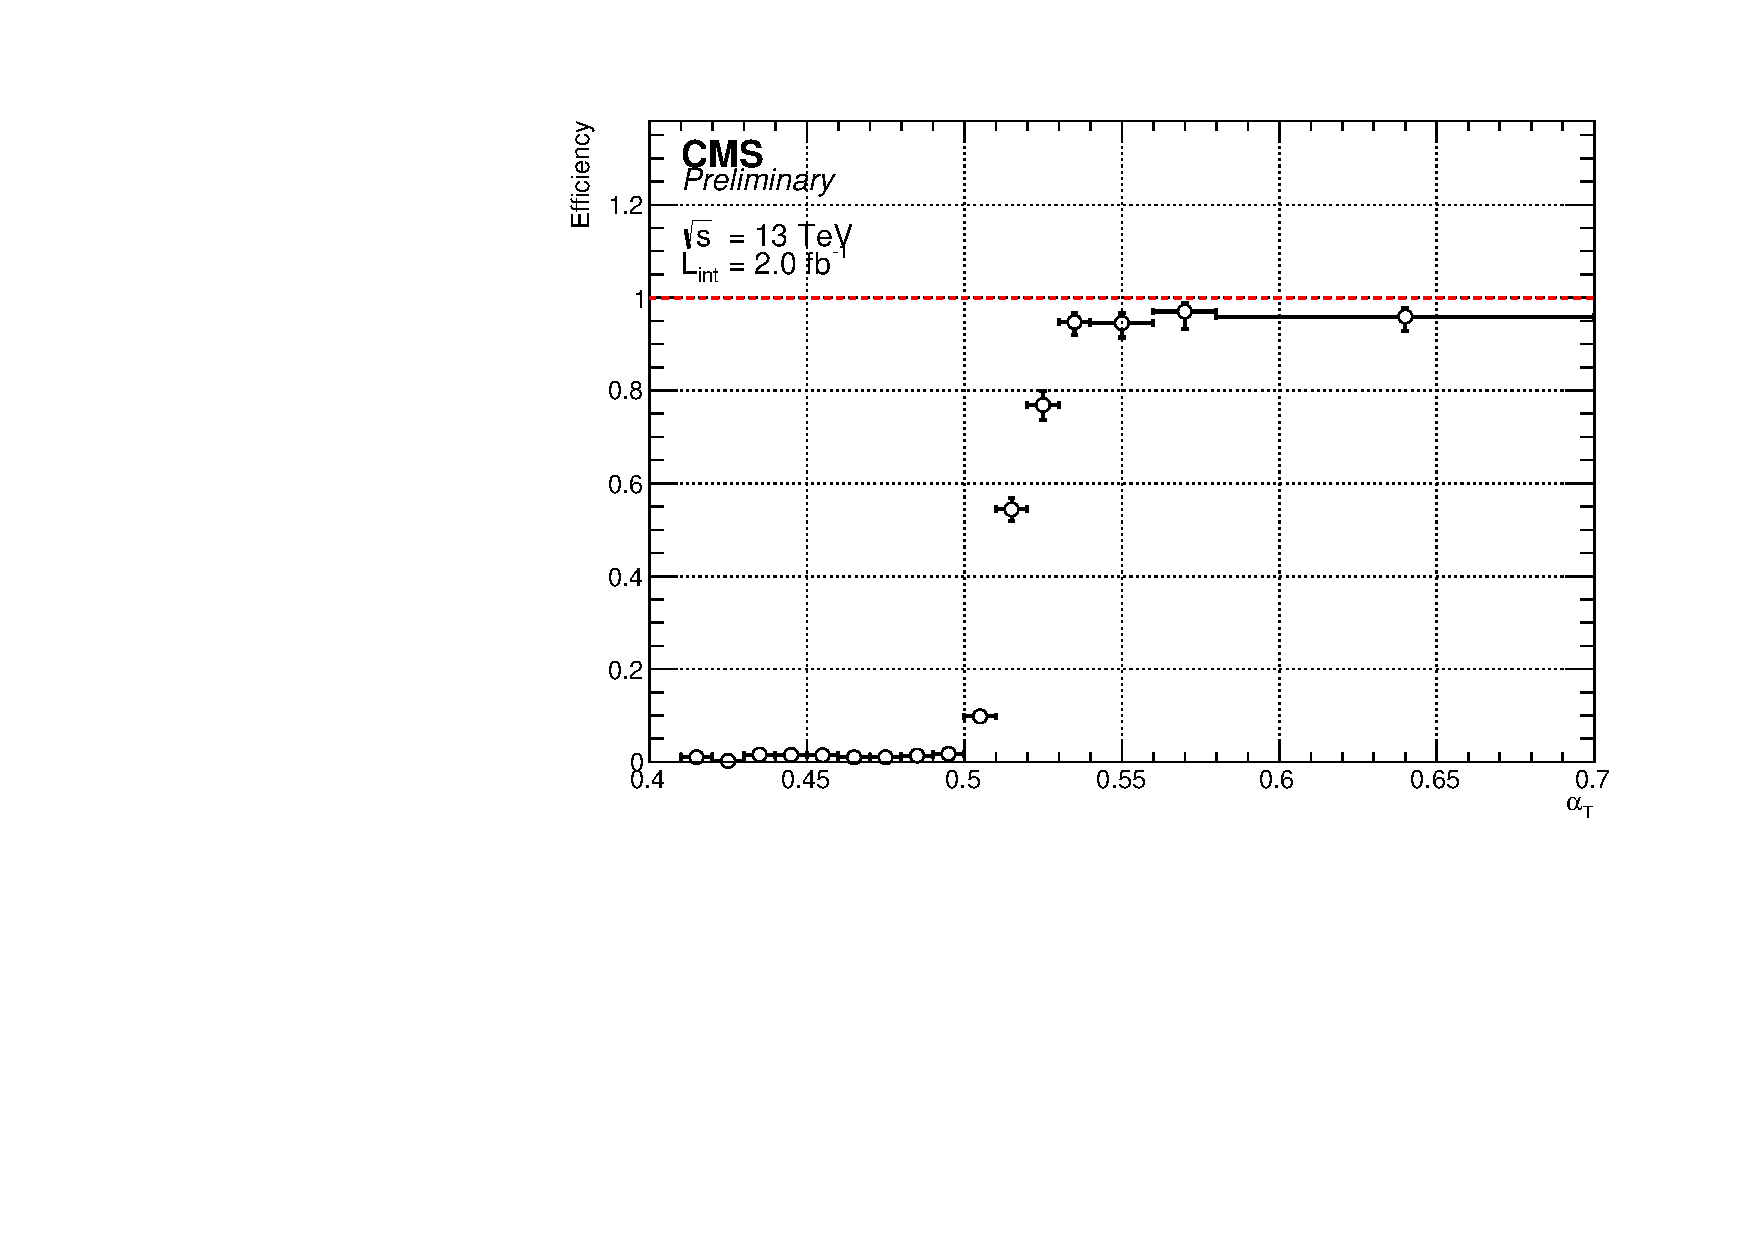
\includegraphics[width=0.5\textwidth]{figures/Trigger/HLT_Ele23_eta2p1_WPLoose_Gsf/HLT_PFHT400_DiPFJetAve90_PFAlphaT0p51_MoM_HT500_alphaT}} ~~
    \subfigure[{\tiny HLT\_PFHT400\_DiPFJetAve90\_PFAlphaT0p51 ($\alt>0.55$)}]{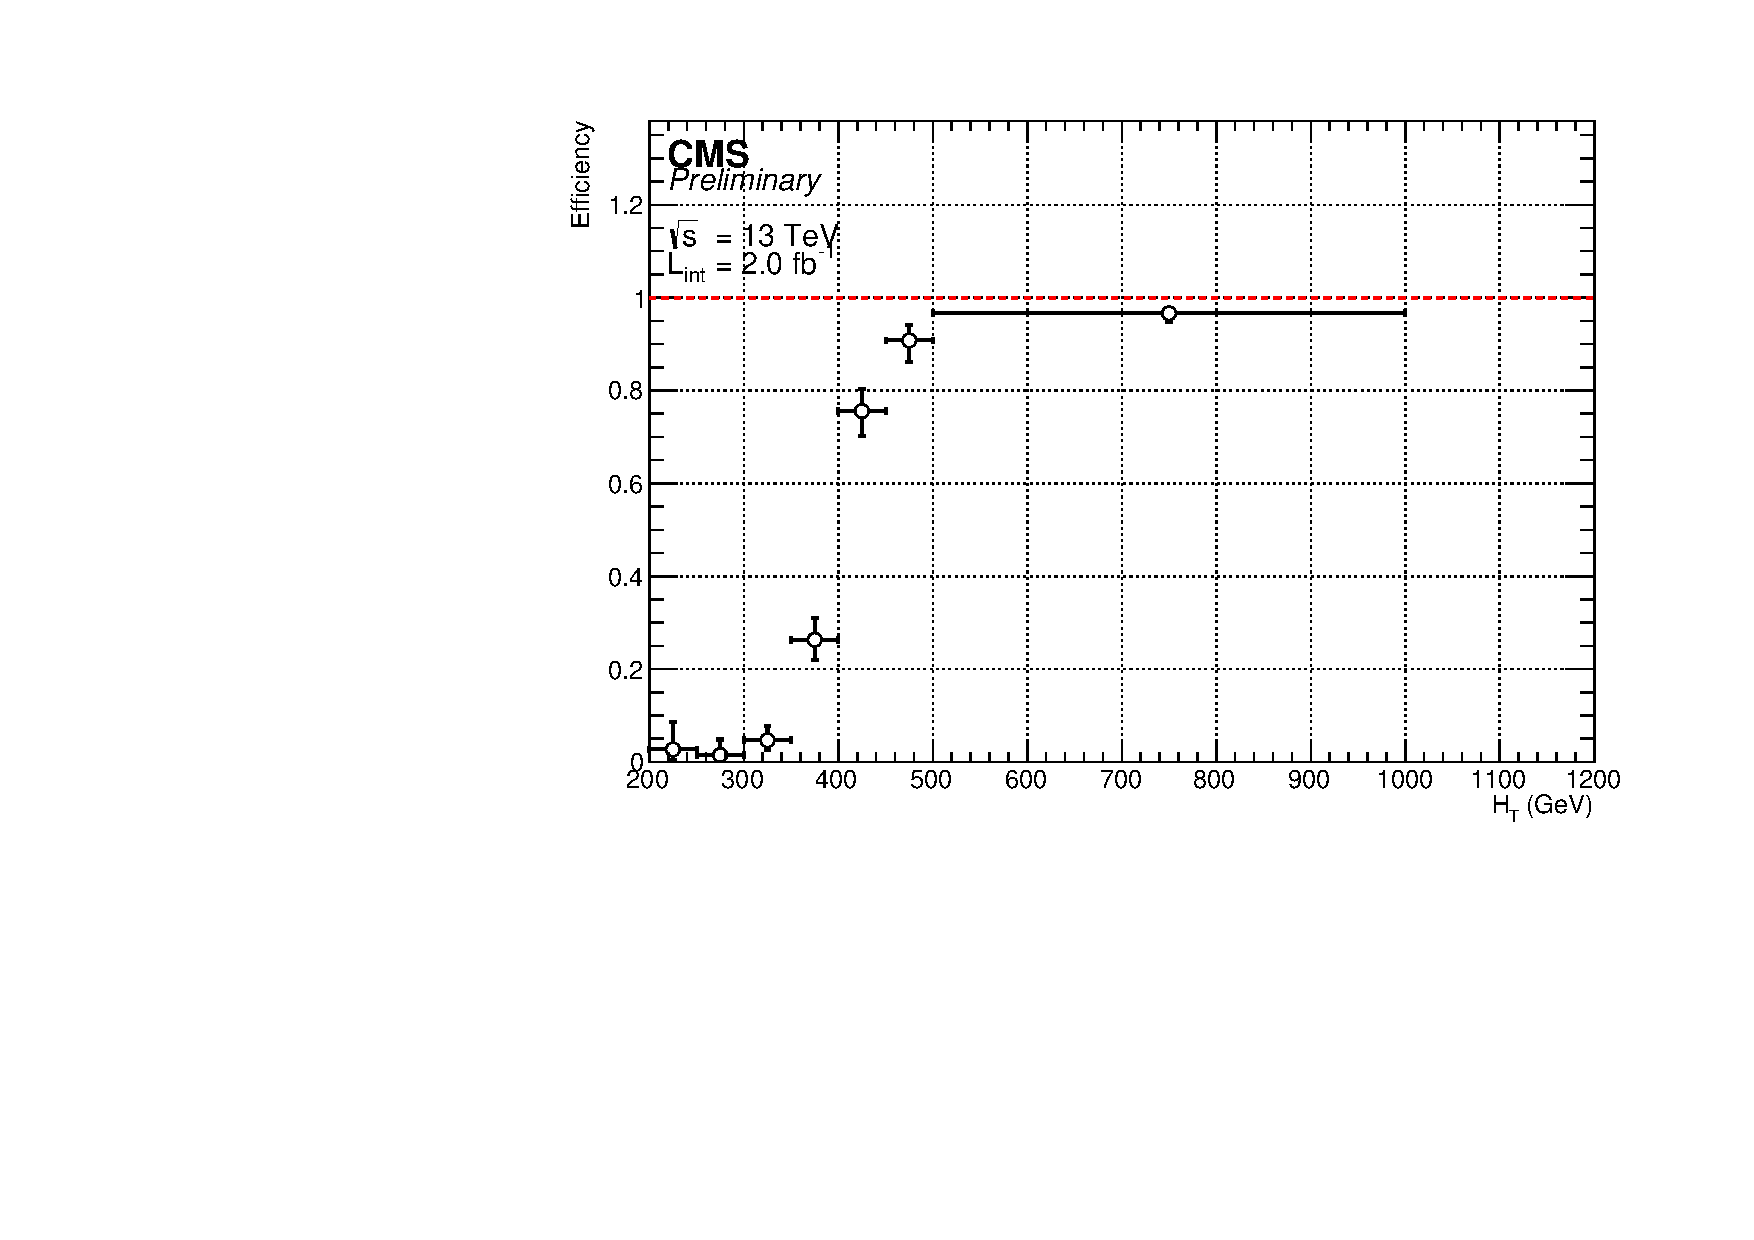
\includegraphics[width=0.5\textwidth]{figures/Trigger/HLT_Ele23_eta2p1_WPLoose_Gsf/HLT_PFHT400_DiPFJetAve90_PFAlphaT0p51_MoM_aT0p55_ht}} ~~
    \caption{
      The trigger efficiency measured in the data as a function of \alt and \scalht in the symmetric categories for the \scalht-\alt triggers used to seed the analysis bins in the signal region. The offline \alt or \scalht cuts applied to ensure full efficiency in the opposite leg are also specified. 
    }
    \label{fig:alphat_turnons}
  \end{center} 
\end{figure}
